\chapter[The 1$^{\text{st}}$ of February 2024 - Architecture of the HiDeNN]{Architecture of the HiDeNN}

\begin{chapabstract}
    The question about a nodal-based or  an element-based architecture is discussed.
\end{chapabstract}

\minitoc

\section{Element-wise architecture}

When moving from linear 1D elements to higher order or dimensions, the use of an element-wise architecture \parencite{liu_hidenn-fem_2023} appears more versatile. The shape functions are therefore built on each element as opposed to globally on the mesh. 

One way of combining those approaches would be to add an \emph{Assembly layer} before the interpolation layer that rebuilds the global shape functions at the structure's (mesh) scale as illustrated in \cref{fig:assembly}.

For each element, a sub-neural network would be built so that the output consists of the local shape functions $\Tilde{N}_i$ defined on the element. 

% \paragraph{Warning} At this point, several versions of the same shape function (associated to the same node) can exist independently through different elements.
\Rq{At this point, several versions of the same shape function (associated to the same node) can exist independently through different elements.}

The \emph{Assembly layer} layer would then reconnect every local version $\Tilde{N}_i$ of a given global shape function $N_i$ associated to the $i-\text{th}$ node of the mesh. This layer would be a linear layer (\textbf{with bias of $-1$}) that inputs all the $\Tilde{N}_i$ and outputs a smaller layer of the $N_i$.
The weight matrix of such a layer would read
\begin{equation}
    w_{i,d\left(e-1\right)+k} = \begin{cases}
        1,\text{ if }k-\text{th node of element }e\text{ is node }i \\
        0,\text{ otherwise}
    \end{cases}
\end{equation}

\begin{figure}[bpt]
    \centering
    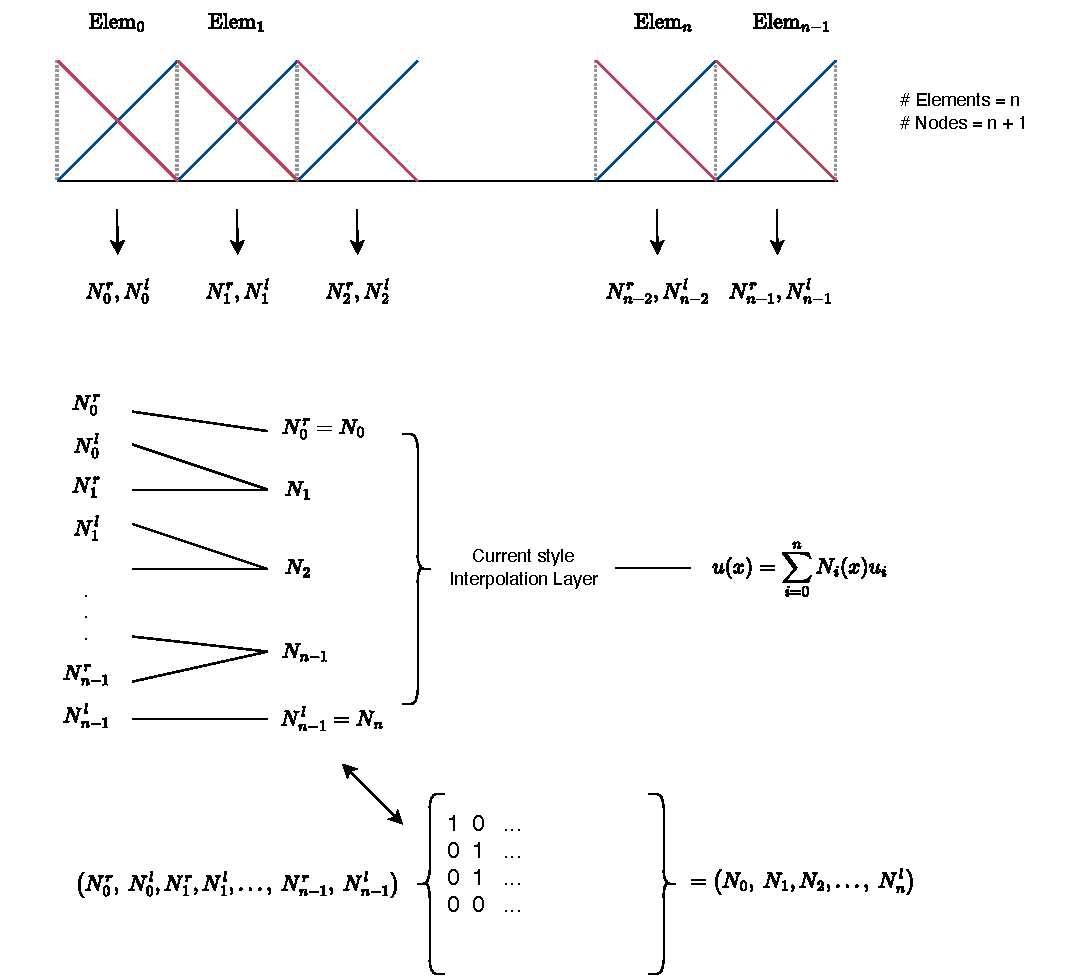
\includegraphics[width = 0.8\linewidth]{Schema/Diagram_NN_elementwise.drawio.pdf}
    \caption{Composition of shape functions.  The operation can be implemented using a linear layer with a weight matrix based on the connectivity table of given mesh and zero bias. This would allow using the existing interpolation layer consisting of nodal values.}
    \label{fig:assembly}
\end{figure}

% \paragraph{Warning}
% When decomposition the shape functions and then assembling them, using an element-wise support for the functions leads to issues on the exact nodal coordinates for the assembled global shape functions as illustrated in \cref{fig:Discontinuous}.


\begin{figure}[htbpt]
    \centering
    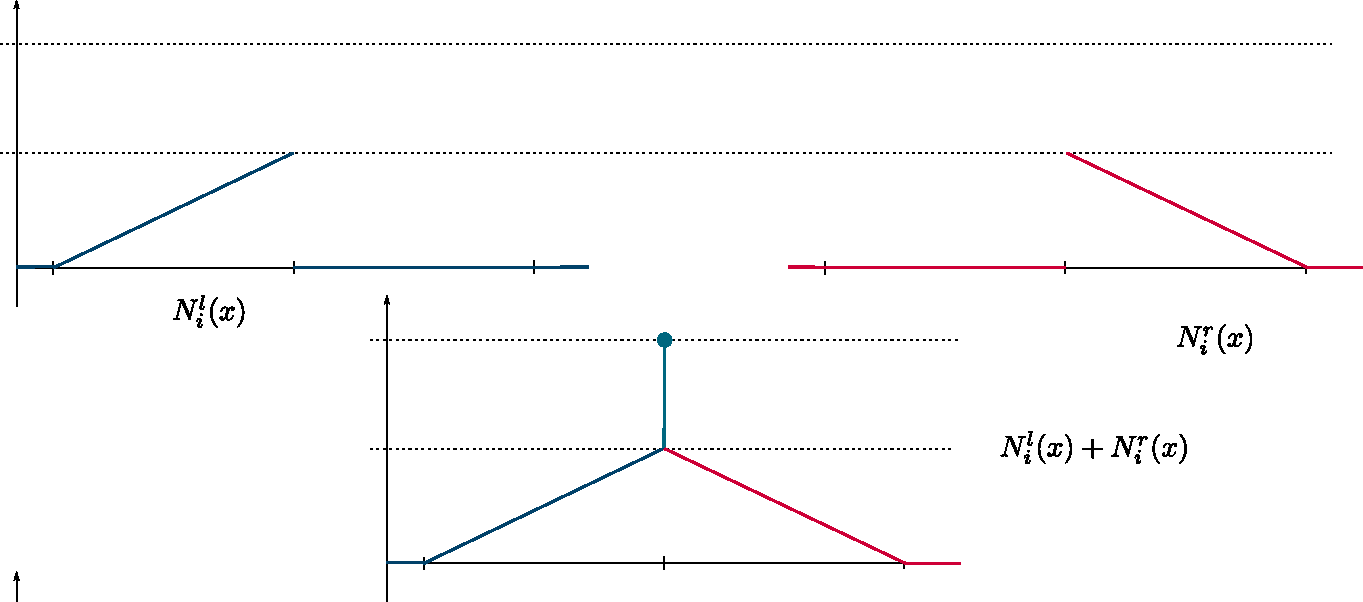
\includegraphics[width=\linewidth]{Schema/Discontinuous_sum.pdf}
    \caption{Element-wise support, discontinuous sum}
    \label{fig:Discontinuous}
\end{figure}
\Rq{When decomposition the shape functions and then assembling them, using an element-wise support for the functions leads to issues on the exact nodal coordinates for the assembled global shape functions as illustrated in \cref{fig:Discontinuous}.
}

Using ``leaking''shape functions that are defined outside of the element \parencite{zhang_hierarchical_2021} allow to bypass this issue as shown in \cref{fig:Continuous}. In that case the assembly layer will need to have the $-1$ biais shown in the last layer of the shape functions detailed by \cite{zhang_hierarchical_2021}.
\begin{itemize}
    \item[\faLightbulb] Check how to apply that idea in higher dimensions
\end{itemize}
\begin{figure}[hbpt]
    \centering
    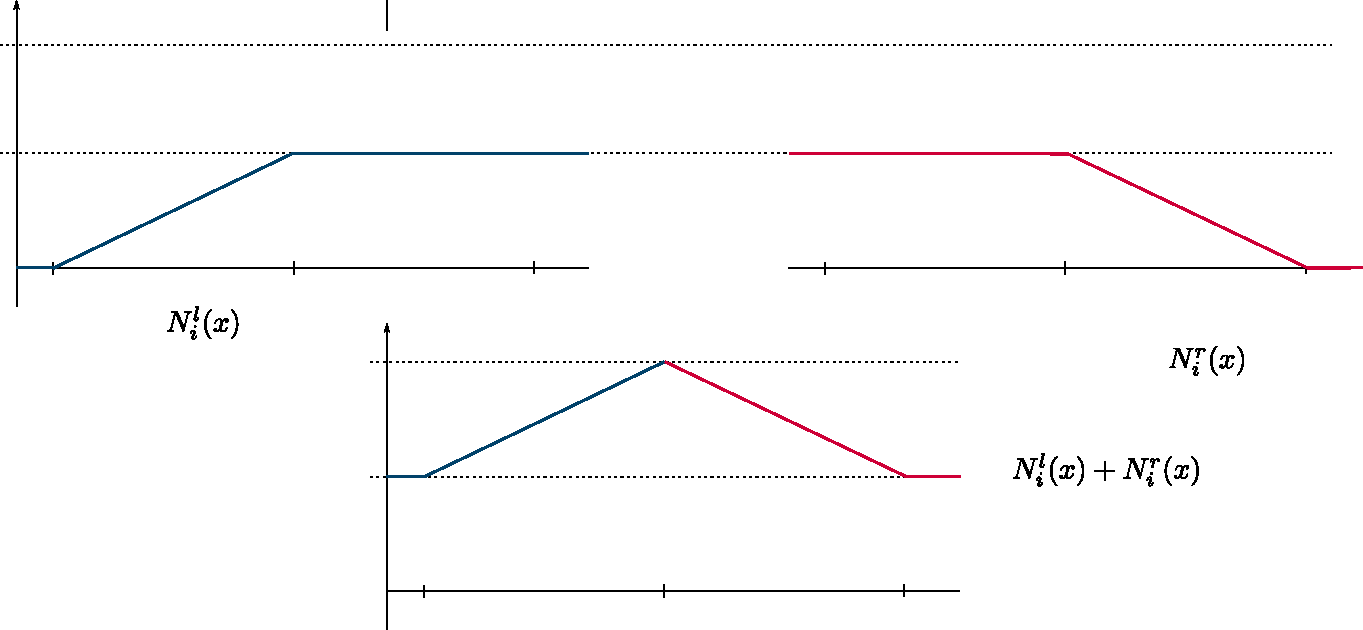
\includegraphics[width=\linewidth]{Schema/Continuous_sum.pdf}
    \caption{Leaking shape functions, continuous sum}
    \label{fig:Continuous}
\end{figure}

\section{Parametric implementation}
The benefits of HiDeNN seem to lie in the parametric capability of such architectures. See \cref{chap:TD}.
\Rq{\begin{itemize}
    \item Feels like without parameters there are no real advantages of HiDeNN over solving the finite element problem
    \begin{itemize}
        \item Maybe in cases where extreme re-meshing is required
    \end{itemize}
    \item With parameters and Tensor Decomposition, the decomposition could be easily automated (might be better than fixed point)
    \begin{itemize}
        \item They sell a parametric version of HiDeNN but so far the only parameters are the 3 spatial parameters (even for HiDeNN-TD) \faChevronRight ~no real ROM yet
    \end{itemize}
    \item Achieve new kind of \emph{a priori} ROM (no snapshots required)
    \item Could get non-linear interpolation relatively "easily"
\end{itemize}}